Während sich agile Praktiken im Hinblick auf die Softwareentwicklung auf eine kontinuierliche Planung, Flexibilität und eine schnelle Reaktion auf sich ändernde Kundenanforderungen fokussieren, können DevOps-Praktiken dazu verwendet werden, den Arbeitsfluss vom Kunden über die Entwicklung, den Betrieb und zurück kontinuierlich auszubauen und damit die Qualität und Belastbarkeit der Software zu steigern. \cite{fitzgerald_continuous_2014} \cite[S. 264]{tokarski_strategische_2018}

Die \textit{'Continuous Everything'}-Methoden spiegeln die Idee einer kontinuierlichen Verbesserung und Automatisierung innerhalb eines Devops-Prozesses wieder. 

Wie in der Abbildung zu erkennen ist, können sich diese Methoden auf merhrere Entwicklungszyklenphasen konzentrieren und werden in diesem Abschnitt im Einzelnen beschrieben.  

\begin{figure}[h]
    \centering
    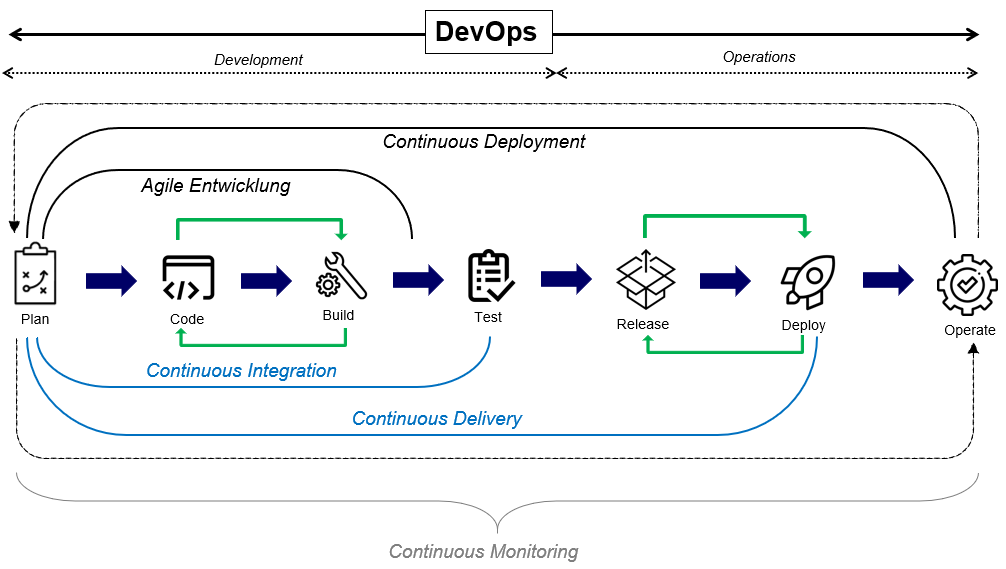
\includegraphics[scale=0.6]{Bilder/Continuous Everything.png}
    \caption{Continuous-Methoden innerhalb des Devops-Lebenszykluses, angelehnt an \cite[S. 16]{halstenberg_devops_2020}}
\end{figure}

\paragraph{Agile Entwicklung}

Die agile Entwicklung beschreibt die Verwendung von agilen Methoden innerhalb des Softwareentwicklungsprozesses als eine wesentliche Grundvoraussetzung für den DevOps-Prozess. 

Oftmals wird dieser Prozess auch als Continuous Planning (dt kontinuierliches Plannen) bezeichnet und reicht von der Phase des Planes bis zur Phase des Builds. \cite{fitzgerald_continuous_2014} 

Wie bereits in der Phase des Planens beschrieben, können agile Methoden wie Scrum und Kanban zum Einsatz kommen um die entsprechenden Ressourcen und die Entwicklungen während des ganzen Zeitraums zu planen und einzuteilen.

Inerhalb dieser Methode werden Features in kleinen Inkrementen geplant und entwickelt, um diese innerhalb eines Sprints umzusetzen und folglich die Durchlaufzeit bis zur Auslieferung kurzzuhalten. \cite[S. 266]{tokarski_strategische_2018} 

Infolgedessen beinhalten die Ergebnisse dieser Methode ausliefbare und getestete Funktionalitäten nach jedem Sprint. 

Continuous Planning gilt als ein ganzheitliches Unterfangen, dass ein engere Intergration zwischen Planung und Ausführung erfordert und an dem sowohl Kunden als auch die Entwickler beteiligt sind. \cite{fitzgerald_continuous_2014} 

Ziel ist es sicherzustellen, dass die Investitionsentscheidungen während des gesamten Lbenszykluses auf die Bedürfnisse des Kunden abgestimmt worden sind. 

\paragraph{Continuous Integration}

Die Methode des Continous Integration (dt. kontinuierliche Integration, kurz: CI) beschreibt grundsätzlich die Gewährleistung einer sicheren und lückenlosen Integration von Codeänderungen in die vorhandenen Umgebungen. \cite[S. 266]{tokarski_strategische_2018}  

Ziel ist es, die Qualität der Software sicherzustellen und schnelles Feedback über die Integrierbarkeit vor der Auslieferung zum Kunden zu erhalten. \cite[S. 266]{tokarski_strategische_2018} 

Kernelement stellt ein Versionsverwaltungssystem (auch: Repository) dar, dessen wesentliche Aufgabe es ist, den DevOps-Teams dabei zu helfen, den Code von mehreren Entwickeln zu organisieren, Änderungen zu verfolgen und automasierte Tests zu ermöglichen. 

Zunächst werden neuer oder geänderter Code nach der Entwicklung und Prüfung regelmäßig und in möglichst kurzen Abständen in einem gemeinsamen Repository gemergt (dt. zusammengeführt). \cite[S. 13-16]{sharma_devops_2017}

In diesem Zuge wird der Code automatisiert in einem Build kompiliert. 

Die neu erstellten Artefakte, als Ergebnis des Builds, werden in eine lauffähige Umgebung integriert und automasiert getestet. 

Damit soll sichergestellt werden, ob die neue Codeänderung einer Komponente im Kontext der gesamten Anwendung lauffähig ist. 

Dies ist essentiell für den Prozess, da häufig viele Entwickler an der Codebasis mit leicht unterschiedlichen Versionen arbeiten und daher überprüft werden kann, ob die verschiedenen Änderungen richtig zusammenarbeiten. \cite[S. 69]{verona_practical_2016} 

Aufgrund des regelmäßigen Integrieren der Codeänderungen wird gewährleistet, dass häufige automatisierte Tests durchführt werden, den Entwicklern stets der aktuellste Code zur Verfügung steht und Entwickler nicht darauf warten müssen, einzelne Codeabschnitte am Tag der Veröffentlichung auf einmal zu integrieren. \cite{thedev_eight_2019} 

Durch die entstehende Flexibilität und Geschwindigkeit können Fehler schneller und leichter behoben werden, da die Programmbestandteile kleiner und weniger komplex sind und das Debugging insgesamt sinkt. \cite{thedev_eight_2019}

Darüber hinaus werden Änderungen sichtbarer und bilden eine starke Grundlage für zukünftige Änderungen. 

Insgesamt umfasst CI Schritte wie die Codekompilierung, die Durchführung von Unit- und Akzeptanztests, die Validierung der Codeabdeckung, die Überprüfung der Einhaltung von Codierungsstandards und die Erstellung von Bereitstellungspaketen. \cite{fitzgerald_continuous_2014} 

\paragraph{Continuous Delivery}

Da regelmäßig Builds durch die Continuous Integration erzeugt werden, müssen diese zeitnah in andere Umgebungen weitergeleitet werden. \cite[S. 16 - 18]{sharma_devops_2017}  

Bei dem Ansatz des Continuous Delivery (dt. kontinuierliches Ausliefern, kurz: CD) handelt es sich um die nächste Stufe des Continuous Integration. 

Die Methode des Continuous Delivery baut auf einer regelmäßigen und automatisierten Bereitstellung des Builds an den Testbereich, zur anschließenden Bewertung und zu einer potentiellen Freigabe an die Kunden, auf. \cite[S. 16 - 18]{sharma_devops_2017}  

Voraussetzung ist der Aufbau einer Continuous-Delivery-Pipeline, zum Ziel das Ausrollen der Software möglichst automatisiert für die Bereitstellung neuer Releases durchzuführen. \cite[S. 10]{wolff_continuous_2016}

Sobald ein neues Artefakt innerhalb des Repositorys übertragen wurde, wird die Continuous-Delivery-Pipeline ausgelöst. \cite[S. 14]{verona_practical_2016} 

In diesem Rahmen werden die fehlerfreien Builds automasiert innerhalb eines produktionsähnlichen Staging- oder Testbereich bereitgestellt, um nach dem Testen zu bewerten, wie sich die Builds produktionsnah verhalten und letztlich in die Produktion verlagert werden können. \cite[S. 16]{sharma_devops_2017}

Falls das Testen in der Pipeline fehlschlägt, werden die Entwickler informiert und haben dmait die Gelegenheit kurzfristig Anpassungen an dem jeweiligen Build vorzunehmen oder diesen zu verwerfen. 

Insgesamt soll sichergestellt werden, dass die neu entstandene Version für den Einsatz im Produktivbetrieb geeignet ist. \cite{thedev_eight_2019}

Das Versionieren in Releases und das Ausliefern der Software wird bei Continuous Delivery möglichst vollständig durch geeignete Tools automatisiert. 

Die Methode des Continuous Delivery beinhaltet mehrere Vorteile für das gesamte DevOps-Team. 

So wird aufgrund des hohen Grades an Automatisierung der Release-Prozess maßgeblich verbessert, indem Risiken und Engpässe durch die häufige Auslieferung von kleinen Features vermieden werden können und damit ein kontinuierlicher Integrationsfluss sichergestellt werden kann. \cite[S. 18]{wolff_continuous_2016}

Zudem sind die Test- und Release-Phasen der Pipeline abgestimmt und ermöglicht es Unternehmen, das Release neuer Builds in beliebigen Abständen manuell auszulösen. \cite{thedev_eight_2019}

\paragraph{Continuous Deployment}

Die letzte Phase der Delivery-Pipeline ist das Continuous Deployment (dt. kontinuierliche Bereitstellung, kurz: CD).

Kernaufgabe des Continuous Deployments ist die voll automatisierte Überführung des Codes in die Produktivumgebung mithilfe der Delivery-Pipeline. \cite[S. 29]{alt_innovationsorientiertes_2017} 

Sowohl Continuous Delivery als auch Continuous Deployment werden in der Literatur oftmals synonym verwendet, da beide auf analoge Konzepte basieren. 

Der Unterschied zwischen beiden Methoden besteht darin, dass Continuous Deployment ein automatisiertes Ausliefern der neuen Version auf die Produktivumgebung beinhaltet, während Continuous Delivery die Auslieferung auf nicht-produktive Umgebungen abzielt. 

Demnach kann das Deployment auf die Produktivumgebung im Rahmen des Continuous Delivery manuell entschieden werden, die widerrum von den fachlichen Erfordernissen des Kunden abhängt. \cite[S. 29 - 30]{alt_innovationsorientiertes_2017} 

Aufgrund der automatisierten Freigabe des Releases, muss sowohl die Qualität als auch die Lauffähigkeit der Pipeline besonders gesichert sein, was wiederrum in der Phase des Continuous Delivery gewährleistet sein muss. \cite[S. 269]{tiemeyer_handbuch_2021} 

Continuous Deployment entspricht demnach dem höchsten Reifegrad einer Delivery-Pipeline, was den DevOps-Teams ermöglicht, kleinste Features und Änderungen für den Anwender ausliefern zu können und wäre theoretisch das höchste Ziel der modernen Softwareentwicklung. \cite{humble_why_2011}  

Durch den höchsten Grad der Automatisierung können die Vorlaufzeiten niedrig gehalten und folglich schnelles Feedback erhalten werden. \cite{humble_why_2011}   

Das Ziel ist es demnach, die Zeit bis zur Markteinführung von der Software zu verkürzen, indem jeder Commit in die Produktivumgebung bereitgestellt wird. 

Viele Entwickler und Unternehmen lehnen die Methode des Continuous Deployments jedoch ab, da es ein Risiko darstellt, wenn eingecheckter Code durch das Testing fehlgeschlagen ist, automasiert in die Produktivumgebung bereitgestellt wird. \cite[S. 269]{tiemeyer_handbuch_2021}  

Um dieses Risiko möglichst gering zu halten, müssen einerseits nahezu produktionsreife Codes und robuste Test-Frameworks vorhanden sein und andererseits alle DevOps-Mechanismen zuverlässig arbeiten. \cite[S. 269]{tiemeyer_handbuch_2021}  

Darüber hinaus verlangt der Continuous-Deployment-Ansatz eine starke Architekturaufsicht und Teamdisziplin, damit das Release nicht die Qualität oder den von den Kunden realisierten Nutzen in Mitleidenschaft zieht.\cite[S. 119 - 120]{erder_continuous_2016} 

An diesem Punkt ist es wichtig, eine Kultur des Vertrauens aufzubauen, die die Zusammenarbeit aller Teamsmitglieder fördert. \cite{humble_why_2011} 

\paragraph{Continuous Monitoring}

Die Vorgehensweise des Continuous Monitoring umfasst die durchgängige Überwachung, der zugrunde liegenden Infrastruktur und des im Betrieb befindlichen Quellcodes. \cite{van_hoorn_continuous_2012} 

Dabei stellt das Ops-Team sicher, dass die Anwendung in der Produktion funktioniert wie gewünscht und die Umgebung stabil läuft. 

Hierfür haben die Ops-Teams eigene Tools zur Überwachung ihrer Umgebung und laufenden Systeme und zwar von der Prozessebene bis hinunter zu Ebenen, die niedriger sind, als es die Systemüberwachungstools erlauben würden. \cite[S. 26]{sharma_devops_2017}

Oftmals werden Selbstüberwachungs- und Analysefunktionen direkt in die zu entwickelnden Anwendungen eingebaut, um eine kontinuierliche End-to-End-Überwachung zu gewährleisten. \cite[S. 26]{sharma_devops_2017}

Neben der Anwendungs- und Systemleistung muss das Benutzerverhalten der Anwendung und die Benutzerzufriedenheit ebenfalls überwacht werden, um ein detalliertes Feedback zu erhalten. \cite[S. 112 - 113]{erder_continuous_2016}

Dieses Feedback kann schnell in die Phase der Entwicklung zurückfließen, um bessere Entscheidungen bei der Entwicklung der nächsten Änderung treffen zu können. 

Auf diese Weise können zusätzliche und neue Anforderungen und Funktionen berücksicht, Probleme behoben und das weitere Vorgehen angepasst werden. 

Sowohl das Feedback als auch Fehler, Probleme oder Ausfälle werden anhand einer Feedbackschleife zurück an die Entwicklung kommuniziert und im besten Fall möglichst zeitnah behoben. \cite[S. 112 - 113]{erder_continuous_2016} 

Im Ergebnis bildet diese Feedbackschleife ein Instrument, zur kontinuierlichen Gestaltung und Orientierung für das Softwareprodukt.   

\paragraph{Infrastructur-as-a-Code}

Obwohl die Vorgehensweise des \textit{Infrastructur-as-a-Code} (kurz: IaC) keine 'Continuous'-Bezeichnung besitzt, ist diese Praktik wesentlicher Bestandteil der gängigen DevOps-Methoden. 

Enstanden ist der IaC-Ansatz zunächst im Bereich des Cloud Computing, als eine Vorraussetzung für automasierte Delivery-Modelle wie IaaS (Infrastructure as a Service). 












Infrastruktur-as-Code steht für Test und Produktionsumgebungen, die komplett automatisiert bereitgestellt und aktualisiert werden
können. Metriken liefern technische und fachliche Informationen zu der in Produktion laufenden
Software: Sie ermöglichen A/B-Tests, um den alten
Prozess parallel zum neuen Prozess zu betreiben und
so aussagekräftige Vergleiche anstellen zu können.
Automatisierung kann dabei Kopfmonopole
verringern und Liegezeiten reduzieren. Allerdings
wird sie nur dann die notwendige Akzeptanz finden, wenn sie zuverlässig und schnell ist – sei es
bei der Installation der Software als auch bei der
Ausführung der Tests.
Übergaben werden mit einer produktzentrierten Organisationsstruktur minimiert: Verschiedene
Produktteams verantworten für ihre jeweiligen Teile
alle Phasen wie fachliches und technisches Design,
Umsetzung, Test, Installation und Betrieb (Abb. 1).
Durch räumliche Nähe und personelle Verflechtung
berücksichtigten sie Erkenntnisse in einer Phase
direkt in anderen Phasen





IaC verfolgt das Ziel einer regelbasierten 
Automatisierung der Installation und Konfguration von virtuellen und physischen Infrastrukturkomponenten wie etwa Server durch Softwareskripte (Spinellis 2012). Im Sinne einer programmierbaren Infrastruktur wird diese zunächst in 
Form von Programmcode abgebildet, um bei der Konfguration ähnliche Tools 
und Mechanismen verwenden zu können, wie beim Deployment von Software. 
Durch Automatisierung lassen sich Konfgurationsprozesse beschleunigen, sie 
gewinnen an Flexibilität, das Fehlerrisiko sinkt im Vergleich zum manuellen Konfgurieren und schließlich dient der Code auch als Dokumentation (Hüttermann 
2012; Ramos 2015). Dazu erfordert IaC die frühzeitige Einbeziehung von Systemadministratoren in den Softwareentwicklungsprozess sowie ein tieferes Verständnis der Entwickler für die Basis-Infrastruktur. Es leistet somit einen Beitrag 
zur engeren Zusammenarbeit von Dev und Ops. Aus Betriebsperspektive besteht 
eine direkte Verwandtschaft zu den Ausprägungen von „Software-defned“-Konzepten, wie etwa Storage, Network oder Datacenter. Für die Realisierung von IaC 
sind mittlerweile leistungsfähige System Confguration Management Toolsets 
wie Puppet oder Chef verfügbar. Ferner unterstützen Cloudanbieter wie Amazon 
(AWS) oder Microsoft (Azure) IaC mit ihren APIs


































Gemäß des DevOps-Konzepts werden die Grundsätze des DevOps-Ansatzes durch den Aufbau einer Bereitstellungspipeline (engl. Deployment Pipeline) durchgesetzt. 

Die Deployment-Pipeline besteht im Wesentlichen aus mehreren Continuous Integration und Continuous Delivery-Pipelines und kann als eine automatisierte Implementierung der Build-, Test-, Deploymment- und Release-Prozesse einer Anwendung definiert werden. 

Mit der Deployment-Pipeline werden drei Ziele verfolgt. \cite[S. 3 - 4]{humble_continuous_2011} 

Zunächst ist jeder Schritt des Prozesses angefangen bei der Erstellung, des Einsatzes, des Testens und der Softwarefreigabe (End-to-End-Prozess) für alle sichtbar, wodurch die gesamte Zusammenarbeit gefördert wird. 

Weiterhin wird das Feedback verbessert, indem die Probleme sehr zeitnah im Prozess erkannt und behoben werden können. 

Darüber hinaus ist es jedem DevOps-Team möglich, alle Softwareversionen in jeder beliebigen Umgebung durch einen vollständig automatisierten Prozess bereitzustellen und freizugeben.






Wie bereits beschrieben ist ein wesentlicher Baustein des DevOps-Konzepts die Automatisierung. 

Oftmals bergen manuelle Arbeiten die Gefahr einer hohen Fehleranfälligkeit, zeitliche Unberechenbarkeit und schwerer Reproduzierung, wodurch insbesondere im Softwarebereitsstellungsprozess wenig Zeit für priorisierte Aufgaben bleiben. 

Um die Rolle der Automatisierung voranzutreiben und zu etablieren, sollten möglichst viele vollautomatisierte Deployments auf die Produktivumgebung aufgesetzt werden.   

In diesem Rahmen müssen DevOps-Teams Deployments. bzw Build-Pipelines aufbauen, um alle Änderungen am System, am Code oder an der Infrastruktur, mittels Pipeline zu automatisieren. 










Eine Deployment-Pipeline ist im Wesentlichen eine automatisierte Implementierung des Build-, Deployment-, Test- und Release-Prozesses Ihrer Anwendung. Jedes Unternehmen wird sich in der Implementierung seiner Deployment-Pipelines unterscheiden, je nach dem Wertstrom für die Freigabe von Software, aber die Prinzipien, die ihnen zugrunde liegen, unterscheiden sich nicht. Ein Beispiel für eine Bereitstellungspipeline ist in Abbildung 1.1 dargestellt.



Die Funktionsweise der Deployment-Pipeline lässt sich wie folgt zusammenfassen. Jede Änderung, die an der Konfiguration, dem Quellcode, der Umgebung oder den Daten einer Anwendung vorgenommen wird, löst die Erstellung einer neuen Instanz der Pipeline aus. 

Einer der ersten Schritte in der Pipeline ist die Erstellung von Binärdateien und Installationsprogrammen. Der Rest der Pipeline führt eine Reihe von Tests mit den Binärdateien durch, um zu beweisen, dass sie freigegeben werden können. 

Jeder Test, den der Freigabekandidat besteht, gibt uns mehr Sicherheit, dass diese bestimmte Kombination aus Binärcode, Konfigurationsinformationen, Umgebung und Daten funktionieren wird. 

Wenn der Freigabekandidat alle Tests besteht, kann er freigegeben werden. Die Deployment-Pipeline hat ihre Grundlage im Prozess der kontinuierlichen Integration und ist im Wesentlichen das Prinzip der kontinuierlichen Integration, das zu seinem logischen Abschluss gebracht wurde. 



